\newpage
\vspace{-.25in}
\section{COMPUTATIONAL READINESS} % typically about 5 pages
\vspace{-.2in}
%Why is nekRS ready for the task? What simulations have we already done?

All simulations proposed here will be performed on GPUs. We propose to use
Summit.  These will be performed with the Nek5000 code
\cite{argonne:nekdoc}, an open-source CFD  community code for the simulation of
unsteady and incompressible or low Mach number fluid flow, heat transfer,
combustion, and magnetohydrodynamics in general three-dimensional domains. We
will in particular use the novel GPU version of Nek5000 - NekRS.

The simulations will be performed using the open source spectral element codes
Nek5000 and NekRS.   {\em Nek5000} is a Gordon Bell prize winning code with a
long development history on leading-edge parallel platforms.  It strong scales
to $>$1M ranks \cite{fischer15} and is currently used by about 400 researchers
around the world for the study of turbulence, heat transfer, combustion, and
other flow phenomena.  {\em NekRS} is a new GPU-oriented version of Nek5000
written in C++ that is being developed as part of DOE's Exascale Computing
Project in the Center for Efficient Exascale Discretizations (CEED).  It is
based on OCCA, the open concurrent compute abstraction developed by Warburton
and co-workers, and uses fast OCCA kernels coming out of Warburton's
libParanumal project.  All simulations on Summit use NekRS, which typically
runs 12--14 times faster than Nek5000 on the Summit nodes because of the
relative performance of the 6 V100s compared to the 42 CPU cores.  (The
principal kernels are sustaining 1-2 Tflops (fp64) on the Nvidia V100s
\cite{fischer20a,warburton2019}.) As part of the CEED mandate, OCCA supports
backends for Nvidia and AMD architectures, so we expect to have state of the
art performance for Frontier as we already do for Summit.

\vspace{-.25in}
\subsection{Use of Resources Requested}
\vspace{-.2in}

The tasks in the project will include numerous cases reflective of different
non-dimensional numbers. The cases are summarized in Table~\ref{tab:cases}.

\begin{table}
\centering
\caption{Summary of cases in the project}
\begin{tabular}{rrrrrr}
\hline
\hline
Task & Max Size ($E$) &  $n$, \# of cases  & $t$, \# of steps & node-hours & Total Storage (TB)\\
\hline
\hline
1 & 5 million       & 12   & 500,000   &    130,000 & 51\\
2 & 6 million       & 4    & 3,000,000 &    210,000 & 40.8\\
3 & 12 million      & 8    & 3,000,000 &    840,000 & 163.2\\
4 & ~90 million  & 6    & 500,000   &  1,170,000 & 459\\
\hline
\hline
\end{tabular}
\label{tab:cases}
\end{table}

The estimates of the max number of degree of freedom are based  on past
experience and the estimated Reynolds numbers. Similar estimates on the number
of time steps to collect statistics are provided. For Tasks 2 and 3,
considerably longer integration times are expected due to either larger scale
separation or the need to collect statistics on a significant number of thermal
fluctuations. All production runs will be performed at polynomial order $N=7$.

As discussed later and presented in Table~\ref{wscaling2} previous weak
calculations have shown that for a 17x17 fuel assembly we can expect a time
step on Summit to cost conservatively 0.7 s for 45,000 elements per node at $N=7$. We
used this data to estimate the number of node-hours
($n\frac{E}{45000}\frac{0.7t}{3600}$).

The total request over 3 years is 2,350,000 node-hours in total. With a 10\% increase to allow for testing and debugging we arrive to 2,584,000 node-hours. Given the milestone table we request:
\begin{itemize}
    \item Year 1, half of the computational request for Task 1 plus one third of the request for Task 2-4, for a total of 885,000 node-hours;
    \item Year 2, half of the computational request for Task 1 plus one third of the request for Task 2-4, for a total of 885,000 node-hours;
    \item Year 3, one third of the request for Task 2-4, for a total of 814,000 node-hours.
\end{itemize}
All simulations are to be conducted on Summit. Almost all our production runs will be performed in the capability queue of Summit and thus can be met only at the OLCF.

In terms of storage we estimate the need to store at least 50 restart files for each case (200 for Task 2 and 3 due to the longer transients) including turbulence budgets. A typical Nek5000 restart files requires 17 GB per 1,000,000 elements. The total estimates for filesystem storage are listed in Table~\ref{tab:cases}. To total for all tasks over 3 years is 714 TB.

Offline storage is estimates at 4 times the total filesystem storage estimate to preserve the  data of previous runs (2.85 PB).

We note that the proposed work is modular and if a reduction in scope is necessary given limited resources,  it can be accomodated by reducing the number of cases for each task.

%Describe your proposed production simulations and state how the runs are tied to each of your project's goals and milestones (Section 4, "Milestone Table"). For the simulations you plan to carry out during production runs, provide a
%\begin{enumerate}[noitemsep,topsep=0pt]
%\item Description of what jobs are going to be run and how they relate to the research/development objectives and milestones given above;
%\item Description of processor/core use for large runs (e.g., 10,000-hour run with 100 cores, or ten 10-hour runs with 10,000 cores, for a 1,000,000-hour allocation).  For the XK7, indicate which of these production simulations employ the GPUs.
%\item Clear, detailed explanation as to how you calculated the requested number of processor hours; and
%\item Summary of your anticipated annual burn rate (e.g., linear or with periods of peak usage).\\
%\end{enumerate}

%\vspace{.1in}
%Also describe the data requirements of your production simulations.  If at any point during your project the sum of your data storage needs in the scratch filesystems exceed 1 petabyte, specific justification is required. For your production simulations, provide a:

%\begin{enumerate}[noitemsep,topsep=0pt]
%\setcounter{enumi}{4}
%\item Estimate and breakdown of the anticipated cumulative size of stored data, in scratch and long-term archival storage, at the end of the requested award.
%\item Description of the effective lifetime of your stored data.  If the lifetime varies, show the breakdown by the total size used.  Explain the reason for the lifetime.
%\item Description of the data, including the expected size of the data, which will be transferred into or out of the center.  Describe what tools for transferring the data from external sources will be used.
%\item Description of the tools for data storage, compression (reduction), and analysis that you currently use. Describe whether the tools and/or applications needed are ready or whether there new capabilities or features that must be developed.
%\item If you are intending to make any fraction of the data generated public, specify:
%\begin{enumerate}[noitemsep,topsep=0pt]
%\item How much data and the scientific purpose
%\item What tool will be used to share the data
%\item From where will the data be shared\\
%\vspace{.1in}
%NOTE: The LCF data management policies can be found at
%
%OLCF:  {\href{https://www.olcf.ornl.gov/computing-resources/data-management/data-management-user-guide/}{https://www.olcf.ornl.gov/computing-resources/data-management/data-management-user-guide/}}
%
%ALCF:  {\href{http://www.alcf.anl.gov/user-guides/data-policy}{http://www.alcf.anl.gov/user-guides/data-policy}}
%\end{enumerate}
%\end{enumerate}

\vspace{-.25in}
\subsection{Computational Approach}
\vspace{-.2in}

In this section we discuss the computational approach of the proposed work based on Nek5000 and NekRS.
%
Nek5000 (1999 Gordon Bell and 2016 R\&D 100 award winning code) is an
open-source simulation-software package that delivers highly accurate solutions
for a wide range of scientific applications including fluid flow, thermal
convection, combustion, and magnetohydrodynamics. It features state-of-the-art,
scalable, high-order algorithms that are fast and efficient on platforms
ranging from laptops to the DOE leadership computing facilities.
({\footnotesize\url{http://nek5000.mcs.anl.gov}})
   Significant applications of Nek5000 include DOE scientific
computing mission areas (reactor, combustion, ocean, wind, etc.) with over 400
users in academia, laboratories, and industry. Its central role in other DOE
projects includes  ECP (CEED, ExaSMR, Urban, Combustion), PSAAP-II, NEUP, NEAMS, NE
High-Impact Project (HIP) and  INL-ANL Center for Thermal Fluid Applications in
Nuclear Energy.
   Active users of Nek5000 are industrial firms AREVA, Westinghouse,
TerraPower, NRG (Energy Research Centre of the Netherlands), and BOSCH, and
universities ETH Zurich, KTH Royal Institute of Technology, ENSAM (Paris),
Texas A\&M, University of Miami, University of Florida, University of Maryland,
Baltimore County, and the University of Illinois Urbana Champaign.

NekRS is a new C++ variant of Nek5000 being developed at Argonne as part of the
ECP Center for Efficient Exascale Discretizations and is the version primarily
used in this work.  It is based
on OCCA and libParanumal, both out of the group of Tim Warburton at
Virginia Tech.  OCCA supports both CUDA and HIP backends (for Nvidia and AMD)
and highly-tuned OCCA kernels that realize roofline-limited performance
(1--2 Tflops, fp64, on the V100) are available in libParanumal \cite{fischer20a}.

\vspace{-.25in}
\subsection{Parallel performance}
\vspace{-.2in}

\paragraph{NekRS: Performance} The baseline performance of NekRS using the current version \cite{tomov2019ecp} is demonstrated here. Figure~\ref{fig:nekrs1} shows performance results on Summit for a 17x17 rod-bundle flow simulation in Figure~\ref{fig:nekrs2}. We started with a mesh using 277,000 elements of order $N=7$ (n=95M grid points total). The Reynolds number is 5000 based on hydraulic diameter. Periodic boundary conditions are used in the axial flow direction and the initial conditions comprise an array of meandering vortices.  Figure~\ref{fig:nekrs1} , left, shows strong scaling results on a few nodes of Summit using NekRS with six V100 GPUs per node or NekRS/Nek5000 with 42 CPUs per node. For the CPU version, NekRS uses Hypre as a coarse grid solver. In this case, NekRS is about 4X slower than Nek5000 because the pressure solver is not yet as optimized as the highly-tuned solver in Nek5000. For the GPU, the NekRS results improve substantially when the coarse grid solver is based on the AMG solver ParAlmond.  Figure~\ref{fig:nekrs1} , center, shows the pressure iteration counts for each of the four cases. Nek5000 uses Schwarz-smoothed p-multigrid; NekRS uses Chebyshev smoothing. When ParAlmond is used for the coarse-grid solve the NekRS iteration counts improve by a factor of two and are on par with those of Nek5000. The Chebyshev smoother requires more work per iteration than the Schwarz-based smoother.  With ongoing effort on the pressure solve we anticipate a 2X reduction in NekRS solution times, which will put it on par with the strong-scaled solution times of Nek5000 with more than 2X energy savings that are already observed for NekRS on Summit's V100s (Figure~\ref{fig:nekrs1} , right).

\begin{figure}[h]
\centering
\includegraphics[width=\textwidth]{../figures/performance_nekrs}
%\includegraphics[width=0.9\textwidth]{./figures/performance_nekrs}
\caption{ NekRS and Nek5000 performance of GPUs vs. CPUs on Summit for turbulent flow simulations with Re=5000 for a 17x17 rod-bundle geometry using total number of grid points $n=95,011,000$. Based on timings from Step 11 to 60, time-per-step with ideal scalings shown as dashed lines (left), pressure iterations per step (center), and dofs-per-joule with respect to time-per-step (right) are shown.}
\label{fig:nekrs1}
\end{figure}

\begin{figure}[h]
\centering
\includegraphics[width=\textwidth]{../figures/fig_1717_2}
%\includegraphics[width=0.8\textwidth]{./figures/fig_1717_2}
\caption{Turbulent flow in a 17x17 rod-bundle computed with NekRS on Summit. Left - Overall view. Right - Detail.}
\label{fig:nekrs2}
\end{figure}

\paragraph{NekRS: Scalability}  We discuss here weak-scaling studies performed on Summit (Oak Ridge National Laboratory). Table~\ref{wscaling} shows the solution times, parallel efficiency, and number of points per rank for the Summit results.  We observe in Table~\ref{wscaling} near-perfect weak-scaling performance up to 2,048 nodes considering 8,000 elements/GPU at $N=7$. The case considered is the DNS of Taylor-Green vortex flow with a triple periodic domain. We report results for 100 time-steps; at 2,048 nodes the runtime was 90 seconds. We note that the performance falls off for GPUs when decreasing the DOF per GPU.

\begin{table} [!h]
\begin{center} \begin{tabular}{ccc}
%\toprule
 \hline
\# of Nodes on Summit & DoF (billion) &  Efficiency on GPUs \\
%\midrule
 \hline
 128  & 3.1  & 1.0   \\
 512  & 12.6 & 0.92  \\
 1024 & 25.2 & 0.88  \\
 2048 & 50.3 & 0.88 \\
 \hline
%\bottomrule
\end{tabular} \end{center}
\caption{\label{wscaling} Taylor-Green Vortices. Weak-scaling on Summit. 8,000 elements per GPU, $N=7$.}
\end{table}

We compare also the performance of the GPU Nek5000 port with the CPU performance on Summit for 1,024 nodes. The same test case was used as for the weak-scaling study: the DNS of Taylor-Green vortices. We performed the simulations with 48,000 elements per node and $N=7$. The CPU simulation was performed with 42 MPI ranks per node, and the GPU simulation was performed with 6 MPI ranks per node. Overall the GPU solver was 11.5 times faster than the standard Nek5000 CPU solver for the same number of nodes.

Table~\ref{wscaling2} shows results for 17x17 assembly calculations (as presented in Figure~\ref{fig:nekrs2}) with increasing mesh counts. The axial length was simply extended while keeping the mesh resolution the same. We note that the time per time-step stabilizes quickly indicating a good weak-scaling performance even for this more complex case.

\begin{table} [!h]
\begin{center} \begin{tabular}{ccc}
%\toprule
 \hline
\# of Nodes on Summit & Elements (Million) &  Average time per time-step \\
%\midrule
 \hline
6	  & 0.277	& 0.312 s \\
66    & 3  	    & 0.455 s \\
264   & 12	    & 0.648 s \\
660   & 30	    & 0.506 s \\
%\bottomrule
\hline
\end{tabular} \end{center}
\caption{\label{wscaling2} 17x17 assembly case. Weak-scaling on Summit. 8,000 elements per GPU, $N=7$.}
\end{table}

\vspace{-.25in}
\subsection{Developmental Work}
\vspace{-.2in}

% For the computational approach described above, describe what, if any, development work has been carried out to-date, especially on the architecture of the requested resource. Describe what development work will be executed during the proposed INCITE campaign and when it will be executed. Provide an estimate of the computational resources required for this work. If applicable, identify the milestones and production activities in Section 2.3.i that are dependent on the developmental work and provide a plan for validating this developmental work.

\vspace{-.15in}
\section{REFERENCES}
\vspace{-.15in}

%References are optional and may be structured in accordance with any style. They {\bf \em {do}} count toward the 15-page limit.


\renewcommand{\section}[2]{}%	No 'References' title
%\renewcommand{\chapter}[2]{}% for other classes


\bibliographystyle{ieeetr}
\bibliography{references,ref_nt,emmd}

\end{document}

